\documentclass{article}
\usepackage{amsmath}
\usepackage{tikz}
\begin{document}

\title{Electricity and Magnetism - Lecture 4 Notes}
\author{Joshua Clement}
\maketitle

\section*{Van der Waals Forces}
\begin{itemize}
    \item \textbf{Induced dipoles} cause weak attractive forces between atoms and molecules.
    \item \textbf{Electron clouds} fluctuate, creating \textbf{temporary dipoles}.
    \item Molecules do not need to be polar to interact.
    \item Fluctuations in electron clouds can synchronize, resulting in \textbf{attractive forces}.
    \item Example: \textbf{Gecko feet} adhere to surfaces via van der Waals forces, allowing them to climb walls.
\end{itemize}

\section*{Insulators vs. Conductors}
\begin{itemize}
    \item \textbf{Insulators}: Electrons are bound to atoms and cannot move freely.
    \begin{itemize}
        \item Examples: plastic, wood, glass, pure water, air.
        \item Electrons can shift slightly but remain bound.
        \item \textbf{Polarization} occurs quickly (less than 1 nanosecond).
    \end{itemize}
    \item \textbf{Conductors}: Charges can move freely.
    \begin{itemize}
        \item Examples: metals, ionic solutions (e.g., NaCl in water).
        \item \textbf{Electric Field Inside a Conductor}: \(E = 0\) in equilibrium.
        \item Charges flow like a liquid; \textbf{mobile charges} can be electrons or ions.
    \end{itemize}
\end{itemize}

\section*{Polarization in Conductors and Insulators}
\begin{itemize}
    \item \textbf{Insulators}: Atoms or molecules polarize individually when an external electric field is applied.
    \item \textbf{Conductors}: The entire \textbf{sea of mobile charges} shifts in response to an external field.
    \item \textbf{Ionic Solutions} (e.g., NaCl in water):
    \begin{itemize}
        \item Positive and negative ions move to either side under an applied electric field (\(E_{\text{app}}\)).
        \item The net electric field (\(E_{\text{net}}\)) results from the applied field and the field due to ion displacement.
    \end{itemize}
\end{itemize}

\section*{Electric Field Inside a Conductor}
\begin{itemize}
    \item \textbf{In Equilibrium}: \(E_{\text{net}} = 0\).
    \item \textbf{Proof by Contradiction}:
    \begin{itemize}
        \item Assume \(E_{\text{net}} \neq 0\). Charges would move, violating equilibrium.
        \item Therefore, \(E_{\text{net}} = 0\) in equilibrium.
    \end{itemize}
    \item Excess charges in a conductor in equilibrium are always found on the \textbf{surface}.
\end{itemize}

\section*{Model of a Metal}
\begin{figure}[h!]
    \centering
    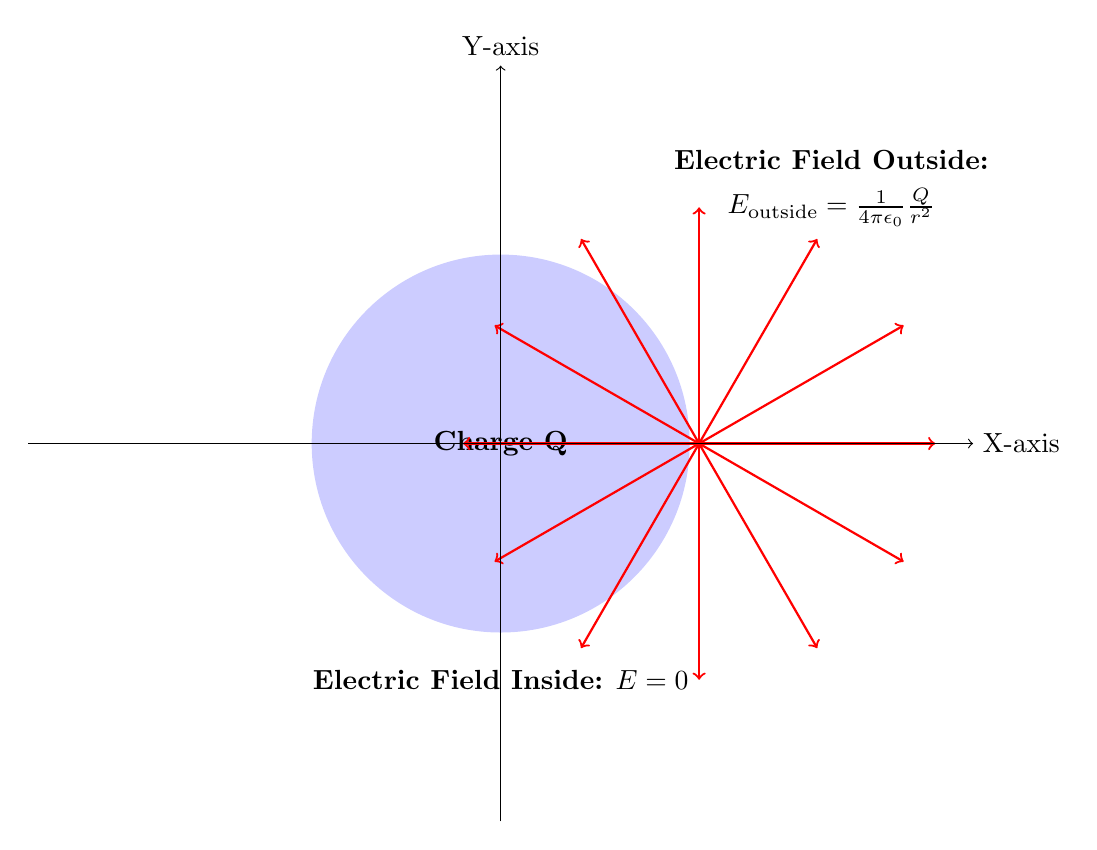
\begin{tikzpicture}[scale=1.2]
        % Draw the sphere
        \fill[blue!20] (0,0) circle (2); % Solid metal sphere

        % Label the sphere
        \node at (0, 0) {\textbf{Charge Q}};

        % Draw the electric field outside the sphere
        \foreach \i in {0, 30, 60, 90, 120, 150, 180, 210, 240, 270, 300, 330} {
            \draw[->, thick, red] (2.1, 0) ++(\i:0) -- ++(\i:2.5) node[pos=1.1, above] {};
        }

        % Draw electric field lines inside the sphere (E = 0)
        \node at (0, -2.5) {\textbf{Electric Field Inside:} $E = 0$};

        % Draw axes for reference
        \draw[->] (-5, 0) -- (5, 0) node[right] {X-axis};
        \draw[->] (0, -4) -- (0, 4) node[above] {Y-axis};

        % Label outside electric field
        \node at (3.5, 3) {\textbf{Electric Field Outside:}};
        \node at (3.5, 2.5) {$E_{\text{outside}} = \frac{1}{4 \pi \epsilon_0} \frac{Q}{r^2}$};

    \end{tikzpicture}
    \caption{Electric field of a solid metal sphere with charge $Q$ in equilibrium. The electric field inside the sphere is $E = 0$, while the electric field outside follows the inverse square law.}
    \label{fig:metal_sphere}
\end{figure}

\begin{figure}[h!]
    \centering
    \begin{tikzpicture}[scale=1.5]
        % Draw the metal sphere
        \fill[gray!30] (0,0) circle (2); % The conducting metal sphere

        % Draw the positive charges on the surface of the sphere
        \foreach \angle in {45, 90, 135, 180, 225, 270, 315, 0} {
            \node[red, scale=1.2] at (2,0) ++(\angle:2) {+};
        }

        % Label inside the sphere for E_net = 0
        \node at (0, 0) {\Large $\vec{E}_{\text{net}} = 0$};

        % Draw the external point charge (-q)
        \fill[blue] (4, 0) circle (0.15);
        \node[right] at (4.2, 0) {\textbf{-q}};


        % Add label for screening effect
        \node[below] at (0, -2.5) {The charges rearrange to cancel the electric field of the point charge (-q)};
    \end{tikzpicture}
    \caption{Conducting sphere with charge +Q near a point charge -q. The charges on the sphere rearrange to screen the field from the point charge.}
    \label{fig:screening_effect}
\end{figure}

\begin{itemize}
    \item \textbf{Mobile electrons} in a metal behave like a liquid and can flow freely.
    \item Metals are good \textbf{conductors} due to this mobile electron sea.
    \item \textbf{Metal Lattice}:
    \begin{itemize}
        \item Atoms form a 3D lattice structure.
        \item Outer electrons are free to move, while inner electrons remain bound to the nucleus.
    \end{itemize}
\end{itemize}

\section*{Charging and Discharging Conductors}
\begin{itemize}
    \item \textbf{Grounding}: Connecting a conductor to a very large object (e.g., Earth) to neutralize its charge.
    \item \textbf{Charging by Induction}:
    \begin{enumerate}
        \item Bring a charged rod close to the conductor.
        \item Ground the conductor.
        \item Break the connection to ground while keeping the rod in place.
        \item Remove the rod, and the conductor retains the induced charge.
    \end{enumerate}
\end{itemize}

\section*{Summary of Conductors vs. Insulators}
\begin{itemize}
    \item \textbf{Conductors}:
    \begin{itemize}
        \item \textbf{Mobile charges} are present.
        \item Entire sea of charges polarizes in an electric field.
        \item In equilibrium: \(E_{\text{net}} = 0\) inside.
        \item Excess charges are only found on the \textbf{surface}.
    \end{itemize}
    \item \textbf{Insulators}:
    \begin{itemize}
        \item No mobile charges.
        \item Individual atoms/molecules polarize.
        \item Inside field: \(E_{\text{net}} \approx E_{\text{app}}\) for low density.
        \item Excess charges can be anywhere in the material.
    \end{itemize}
\end{itemize}

\end{document}